%% The first command in your LaTeX source must be the \documentclass command.
%%
%% Options:
%% twocolumn : Two column layout.
%% hf: enable header and footer.
\documentclass[
% twocolumn,
% hf,
]{ceurart}

\usepackage{tikz}

%%
%% One can fix some overfulls
\sloppy

%%
%% Minted listings support 
%% Need pygment <http://pygments.org/> <http://pypi.python.org/pypi/Pygments>
\usepackage{minted}
%% auto break lines
\setminted{breaklines=true}


% Color definitions
\definecolor{customorange}{rgb}{0.94, 0.55, 0}
\definecolor{customteal}{rgb}{0.47, 0.52, 0.6}
\definecolor{customgreen}{rgb}{0.18, 0.62, 0.27}
\definecolor{fontcolor}{rgb}{0.204, 0.227, 0.251}

\tikzstyle{parentbox} = [rectangle, rounded corners=1mm]
\tikzstyle{parentarrow} = [-stealth, line width=0.5mm]

%%
%% end of the preamble, start of the body of the document source.
\begin{document}


%%
%% Rights management information.
%% CC-BY is default license.
\copyrightyear{2024}
\copyrightclause{Copyright for this paper by its authors.
  Use permitted under Creative Commons License Attribution 4.0
  International (CC BY 4.0).}

%%
%% This command is for the conference information            %%%%%%% TODO !!! UPDATE THIS %%%%%%
\conference{Woodstock'22: Symposium on the irreproducible science,
  June 07--11, 2022, Woodstock, NY}

%%
%% The "title" command
\title{A better way to format your document for CEUR-WS}

% Authors
\author[1]{Darren Rawlings}[%
email=abc@def.ghi,
url=https://startung.github.io/,
]
\address[1]{University of Groningen, Broerstraat 5, 9712 CP Groningen, Netherlands}

\author[]{Tim Chopard}[%
email=timchopard@pm.me,
url=http://cloudberries.io,
]

\fntext[1]{These authors contributed equally.}

%%
%% The abstract is a short summary of the work to be presented in the
%% article.
\begin{abstract}
  A clear and well-documented \LaTeX{} document is presented as an
  article formatted for publication by CEUR-WS in a conference
  proceedings. Based on the ``ceurart'' document class, this article
  presents and explains many of the common variations, as well as many
  of the formatting elements an author may use in the preparation of
  the documentation of their work.
\end{abstract}

%%
%% Keywords. The author(s) should pick words that accurately describe
%% the work being presented. Separate the keywords with commas.
\begin{keywords}
  Multi-Label classification\sep
  Principal component analysis\sep
  ResNet\sep
  Vision Transformers\sep
  XGBoost\sep
  GeoLifeCLEF 2024\sep
  CEUR-WS
\end{keywords}

%%
%% This command processes the author and affiliation and title
%% information and builds the first part of the formatted document.
\maketitle
\section{Introduction}
\section{Method}

In order to manage the multilabel classification required for this research we implemented an ensemble approach. 
This section details the individual architectures and the methods used to combine them.

\subsection{Architectures}

The core architectures used in this project were 18 layer ResNet, XGBoost and [TRANSFORMER]. The outputs of these were 
then weighted and combined before the maximum arguments were selected.

\subsubsection{Principal Component Analysis}
Principal Component Analysis (PCA) is a method for reducing dimensionality~\cite{pcapaper}. It functions by projecting the high dimensional data onto the direction of maximum variance, thus retaining key features and reducing noise.



\subsubsection{XGBoost}
XGBoost is an open source gradient tree boosting package~\cite{xgboost}. 
For this research we used the xgbregression model It has shown broad success accross a range of tasks, performing on par with or better than most equivalent and Automated Machine learning approaches~\cite{xgbcomp}.
\subsubsection{ResNet}
ResNet (Residual Network) is an architecture for deep neural networks that speeds up the training process through the use of residual connections~\cite{resnet}. 
For the purposes of this research we focused on ResNet18, the 18 layer deep variation with some modifications to accomodate the shape of the input data and the required output. 
\subsubsection{[Transformer]}

\subsection{Process}

\subsubsection{Preprocessing}

The raw data included some missing, or infinite values that needed to be processed prior to model fitting. When a column was both deemed important to model fitting and contained such values, these values were replaced by the mean so as to avoid excessive influence from outliers without overly effecting the shape of the data~\cite{missingmedian}.

The Metadata and Bioclimatic Rasters were preprocessed for use in the count and XGBoost models in order to both reduce dimensionality and remove potential noise.




In addition, the number of viable output species was reduced from 11255 (the total species present accross all data) down to 1141 (the total species with more than 100 occurrences in the presence/absence data). 
This reduction served to remove several edge cases and focus the models more on likelier species.

\begin{figure}\label{fig:preproc}
    \begin{center}
        \tikzstyle{databox} = [parentbox, minimum width=40mm, minimum height=12mm, text centered, draw=red!70, fill=red!10, text=fontcolor!70]
\tikzstyle{pcabox} = [parentbox, minimum width=20mm, minimum height=7mm, text centered, draw=customorange!70, fill=customorange!10, text=fontcolor!70]
\tikzstyle{sarrowxgb} = [parentarrow, draw=customorange!70]
\tikzstyle{outbox} = [parentbox, minimum width=40mm, minimum height=12mm, text centered, draw=blue!70, fill=blue!10, text=fontcolor!70]
\tikzstyle{sarrowout} = [parentarrow, draw=blue!50]


\begin{tikzpicture}

    
% Data
\node (bioclim) [databox] {Bioclimatic Rasters};
% \node (landsat) [databox, below of=bioclim, yshift=-7mm] {LandSat};
\node (metadata) [databox, below of=bioclim, yshift=-7mm] {Metadata};
% \node (sentinel) [databox, below of=metadata, yshift=-7mm] {Sentinel};
    

% PCAs
\node (pca0) [pcabox, right of=bioclim, xshift=30mm, yshift=15mm] {PCA$_0$}; 
\node (pca1) [pcabox, below of=pca0] {PCA$_1$}; 
\node (vertellipsis0) [below of=pca1, yshift=3mm] {\Large{\textcolor{fontcolor!70}{$\cdot$}}};
\node (vertellipsis1) [below of=vertellipsis0, yshift=9mm] {\Large{\textcolor{fontcolor!70}{$\cdot$}}};
\node (vertellipsis2) [below of=vertellipsis1, yshift=9mm] {\Large{\textcolor{fontcolor!70}{$\cdot$}}};
\node (pca2) [pcabox, below of=vertellipsis2, yshift=3mm] {PCA$_n$}; 
\draw[sarrowxgb] (bioclim.east) .. controls +(right:5mm) and +(left:8mm) .. (pca0.west);
\draw[sarrowxgb] (bioclim.east) .. controls +(right:5mm) and +(left:8mm) .. (pca1.west);
\draw[sarrowxgb] (bioclim.east) .. controls +(right:5mm) and +(left:8mm) .. (pca2.west);

\node (output) [outbox, right of=pca1, xshift=40mm, yshift=-15mm] {Processed Data};

\draw[sarrowout] (pca0.east) .. controls +(right:5mm) and +(left:8mm) .. (output.west);
\draw[sarrowout] (pca1.east) .. controls +(right:5mm) and +(left:8mm) .. (output.west);
\draw[sarrowout] (pca2.east) .. controls +(right:5mm) and +(left:8mm) .. (output.west);
\draw[sarrowout] (metadata.east) .. controls +(right:60mm) and +(left:10mm) .. (output.west);


% \node (baseens) [baseens, right of=bioclim, yshift=-43mm, xshift=40mm] {Score Ensemble};
% \draw[sarrowxgb] (bioclim.east) .. controls +(right:5mm) and +(left:8mm) .. (baseens.west);
% \draw[sarrowxgb] (landsat.east) .. controls +(right:5mm) and +(left:8mm) .. (baseens.west);
% \draw[sarrowxgb] (metadata.east) .. controls +(right:5mm) and +(left:8mm) .. (baseens.west);
% \draw[sarrowxgb] (sentinel.east) .. controls +(right:5mm) and +(left:8mm) .. (baseens.west);



\end{tikzpicture} 
        \caption{Preprocessing the data for use in the count prediction and XGBoost pseudo-probability models}
    \end{center}
\end{figure}



\subsubsection{Main Process}
\newcommand{\nspecies}{N_{\text{species}}}

There were two key steps to the process of species selection. First the core models which generated pseudo-probabilities and were then weighted and combined. 
Second separeate models were used to determine the expected number $(\nspecies)$ of species per survey. 
These steps came together with the expected counts being used to select the top  $\nspecies$ psuedo-probabilities per survey.

% \subsubsection{Species scoring}
% \begin{figure}
%     \begin{center}
%         % Tikz shape definitions
\tikzstyle{nnbox} = [rectangle, rounded corners=0.5mm, minimum width=35mm, minimum height=10mm, text centered, draw=customteal, fill=customteal!30, text=fontcolor]
\tikzstyle{transformerbox} = [rectangle, rounded corners=0.5mm, minimum width=35mm, minimum height=10mm, text centered, draw=customgreen, fill=customgreen!30, text=fontcolor]
\tikzstyle{xgbbox} = [rectangle, rounded corners=0.5mm, minimum width=35mm, minimum height=10mm, text centered, draw=customorange, fill=customorange!30, text=fontcolor]
\tikzstyle{pcabox} = [rectangle, rounded corners=2mm, minimum width=20mm, minimum height=7mm, text centered, draw=customorange!70, fill=customorange!10, text=fontcolor!70]
\tikzstyle{databox} = [rectangle, minimum width=40mm, minimum height=12mm, text centered, draw=red!70, fill=red!10, text=fontcolor!70]
\tikzstyle{convnode} = [rectangle, rounded corners=3mm, minimum width=6mm, minimum height=6mm, fill=customteal!40, draw=customteal!80]
\tikzstyle{output} = [rectangle, minimum width=30mm, minimum height=10mm, fill=blue!20, draw=blue!50]
\tikzstyle{sarrowxgb} = [->, thick, draw=customorange!70]
\tikzstyle{sarrownn} = [->, thick, draw=customteal!70]
\tikzstyle{sarrowtr} = [->, thick, draw=customgreen!70]
\tikzstyle{sarrowout} = [->, thick, draw=blue!50]


\begin{tikzpicture}

% Data
\node (bioclim) [databox] {Bioclimatic Rasters};
\node (landsat) [databox, below of=bioclim, yshift=-7mm] {LandSat};
\node (metadata) [databox, below of=landsat, yshift=-7mm] {Metadata};
\node (sentinel) [databox, below of=metadata, yshift=-7mm] {Sentinel};

% PCAs
\node (pca0) [pcabox, right of=bioclim, xshift=30mm, yshift=30mm] {PCA$_0$}; 
\node (pca1) [pcabox, below of=pca0] {PCA$_1$}; 
\node (vertellipsis0) [below of=pca1, yshift=3mm] {\Large{\textcolor{fontcolor!70}{$\cdot$}}};
\node (vertellipsis1) [below of=vertellipsis0, yshift=9mm] {\Large{\textcolor{fontcolor!70}{$\cdot$}}};
\node (vertellipsis2) [below of=vertellipsis1, yshift=9mm] {\Large{\textcolor{fontcolor!70}{$\cdot$}}};
\node (pca2) [pcabox, below of=vertellipsis2, yshift=3mm] {PCA$_n$}; 
\draw[sarrowxgb] (bioclim.east) .. controls +(right:5mm) and +(left:8mm) .. (pca0.west);
\draw[sarrowxgb] (bioclim.east) .. controls +(right:5mm) and +(left:8mm) .. (pca1.west);
\draw[sarrowxgb] (bioclim.east) .. controls +(right:5mm) and +(left:8mm) .. (pca2.west);

% XGB
\node (xgb) [xgbbox, right of=pca0, xshift=30mm, yshift=-15mm] {XGBoostRegressor};
\draw[sarrowxgb] (pca0.east) .. controls +(right:5mm) and +(left:8mm) .. (xgb.west);
\draw[sarrowxgb] (pca1.east) .. controls +(right:5mm) and +(left:8mm) .. (xgb.west);
\draw[sarrowxgb] (pca2.east) .. controls +(right:5mm) and +(left:8mm) .. (xgb.west);
\draw[sarrowxgb] (landsat.east) .. controls +(right:35mm) and +(left:10mm) .. (xgb.west);
\draw[sarrowxgb] (metadata.east) .. controls +(right:35mm) and +(left:10mm) .. (xgb.west);

% ResNet
\node (nn0) [nnbox, below of=xgb, yshift=-15mm] {ResNet18};
\node (nn1) [nnbox, below of=nn0, yshift=-3mm] {ResNet18};
\node (nn2) [nnbox, below of=nn1, yshift=-3mm] {ResNet18};
\node (conv) [convnode, right of=nn1, xshift=20mm] {};
\draw[sarrownn] (bioclim.east) .. controls +(right:25mm) and +(left:20mm) .. (nn0.west);
\draw[sarrownn] (landsat.east) .. controls +(right:25mm) and +(left:20mm) .. (nn1.west);
\draw[sarrownn] (sentinel.east) .. controls +(right:25mm) and +(left:20mm) .. (nn2.west);
\draw[sarrownn] (nn0.east) .. controls +(right:7mm) and +(left:7mm) .. (conv.west);
\draw[sarrownn] (nn1.east) .. controls +(right:7mm) and +(left:7mm) .. (conv.west);
\draw[sarrownn] (nn2.east) .. controls +(right:7mm) and +(left:7mm) .. (conv.west);

% Transformer
\node (transformer) [transformerbox, below of=nn2, yshift=-15mm] {Transformer};
\draw[sarrowtr] (bioclim.east) .. controls +(right:25mm) and +(left:20mm) .. (transformer.west);
\draw[sarrowtr] (landsat.east) .. controls +(right:25mm) and +(left:20mm) .. (transformer.west);
\draw[sarrowtr] (metadata.east) .. controls +(right:25mm) and +(left:20mm) .. (transformer.west);
\draw[sarrowtr] (sentinel.east) .. controls +(right:25mm) and +(left:20mm) .. (transformer.west);

% Output
\node (output) [output, right of=transformer, xshift=30mm, yshift=-15mm] {Output};
\draw[sarrowout] (xgb.east) .. controls +(right:25mm) and +(north:50mm) .. (output.north);
\draw[sarrowout] (conv.east) .. controls +(right:5mm) and +(north:20mm) .. (output.north);
\draw[sarrowout] (transformer.east) .. controls +(right:15mm) and +(north:10mm) .. (output.north);

\end{tikzpicture}
%         \caption{The structure of the scoring ensemble from data through to individual species score outputs.}
%     \end{center}\label{fig:score-structure}
% \end{figure}
% \subsubsection{Species counts}
% \begin{figure}
%     \begin{center}
%         % Tikz shape definitions
\tikzstyle{parentbox} = [rectangle, rounded corners=1mm] % TODO
\tikzstyle{nnbox} = [parentbox, minimum width=35mm, minimum height=10mm, text centered, draw=customteal, fill=customteal!30, text=fontcolor]
\tikzstyle{transformerbox} = [parentbox, minimum width=35mm, minimum height=10mm, text centered, draw=customgreen, fill=customgreen!30, text=fontcolor]
\tikzstyle{xgbbox} = [parentbox, minimum width=35mm, minimum height=10mm, text centered, draw=customorange, fill=customorange!30, text=fontcolor]
\tikzstyle{pcabox} = [parentbox, minimum width=20mm, minimum height=7mm, text centered, draw=customorange!70, fill=customorange!10, text=fontcolor!70]
\tikzstyle{databox} = [parentbox, minimum width=40mm, minimum height=12mm, text centered, draw=red!70, fill=red!10, text=fontcolor!70]
\tikzstyle{convnode} = [rectangle, rounded corners=3mm, minimum width=6mm, minimum height=6mm, fill=customteal!40, draw=customteal!80]
\tikzstyle{output} = [parentbox, minimum width=30mm, minimum height=10mm, fill=blue!20, draw=blue!50]

\tikzstyle{baseens} = [parentbox, minimum height=30mm, minimum height=20mm, fill=customorange!30, draw=customorange!70]

% Arrows
\tikzstyle{parentarrow} = [-stealth, line width=0.5mm]
\tikzstyle{sarrowxgb} = [parentarrow, draw=customorange!70]
\tikzstyle{sarrownn} = [parentarrow, draw=customteal!70]
\tikzstyle{sarrowtr} = [parentarrow, draw=customgreen!70]
\tikzstyle{sarrowout} = [parentarrow, draw=blue!50]


\begin{tikzpicture}

    
% Data
\node (bioclim) [databox] {Bioclimatic Rasters};
\node (landsat) [databox, below of=bioclim, yshift=-7mm] {LandSat};
\node (metadata) [databox, below of=landsat, yshift=-7mm] {Metadata};
\node (sentinel) [databox, below of=metadata, yshift=-7mm] {Sentinel};
    
\node (baseens) [baseens, right of=bioclim, yshift=-43mm, xshift=40mm] {Score Ensemble};
\draw[sarrowxgb] (bioclim.east) .. controls +(right:5mm) and +(left:8mm) .. (baseens.west);
\draw[sarrowxgb] (landsat.east) .. controls +(right:5mm) and +(left:8mm) .. (baseens.west);
\draw[sarrowxgb] (metadata.east) .. controls +(right:5mm) and +(left:8mm) .. (baseens.west);
\draw[sarrowxgb] (sentinel.east) .. controls +(right:5mm) and +(left:8mm) .. (baseens.west);


    % % PCAs
% \node (pca0) [pcabox, right of=bioclim, xshift=30mm, yshift=30mm] {PCA$_0$}; 
% \node (pca1) [pcabox, below of=pca0] {PCA$_1$}; 
% \node (vertellipsis0) [below of=pca1, yshift=3mm] {\Large{\textcolor{fontcolor!70}{$\cdot$}}};
% \node (vertellipsis1) [below of=vertellipsis0, yshift=9mm] {\Large{\textcolor{fontcolor!70}{$\cdot$}}};
% \node (vertellipsis2) [below of=vertellipsis1, yshift=9mm] {\Large{\textcolor{fontcolor!70}{$\cdot$}}};
% \node (pca2) [pcabox, below of=vertellipsis2, yshift=3mm] {PCA$_n$}; 
% \draw[sarrowxgb] (bioclim.east) .. controls +(right:5mm) and +(left:8mm) .. (pca0.west);
% \draw[sarrowxgb] (bioclim.east) .. controls +(right:5mm) and +(left:8mm) .. (pca1.west);
% \draw[sarrowxgb] (bioclim.east) .. controls +(right:5mm) and +(left:8mm) .. (pca2.west);

% % XGB
% \node (xgb) [xgbbox, right of=pca0, xshift=30mm, yshift=-15mm] {XGBoostRegressor};
% \draw[sarrowxgb] (pca0.east) .. controls +(right:5mm) and +(left:8mm) .. (xgb.west);
% \draw[sarrowxgb] (pca1.east) .. controls +(right:5mm) and +(left:8mm) .. (xgb.west);
% \draw[sarrowxgb] (pca2.east) .. controls +(right:5mm) and +(left:8mm) .. (xgb.west);
% \draw[sarrowxgb] (landsat.east) .. controls +(right:35mm) and +(left:10mm) .. (xgb.west);
% \draw[sarrowxgb] (metadata.east) .. controls +(right:35mm) and +(left:10mm) .. (xgb.west);

% % ResNet
% \node (nn0) [nnbox, below of=xgb, yshift=-15mm] {ResNet18};
% \node (nn1) [nnbox, below of=nn0, yshift=-3mm] {ResNet18};
% \node (nn2) [nnbox, below of=nn1, yshift=-3mm] {ResNet18};
% \node (conv) [convnode, right of=nn1, xshift=20mm] {};
% \draw[sarrownn] (bioclim.east) .. controls +(right:25mm) and +(left:20mm) .. (nn0.west);
% \draw[sarrownn] (landsat.east) .. controls +(right:25mm) and +(left:20mm) .. (nn1.west);
% \draw[sarrownn] (sentinel.east) .. controls +(right:25mm) and +(left:20mm) .. (nn2.west);
% \draw[sarrownn] (nn0.east) .. controls +(right:7mm) and +(left:7mm) .. (conv.west);
% \draw[sarrownn] (nn1.east) .. controls +(right:7mm) and +(left:7mm) .. (conv.west);
% \draw[sarrownn] (nn2.east) .. controls +(right:7mm) and +(left:7mm) .. (conv.west);

% % Transformer
% \node (transformer) [transformerbox, below of=nn2, yshift=-15mm] {Transformer};
% \draw[sarrowtr] (bioclim.east) .. controls +(right:25mm) and +(left:20mm) .. (transformer.west);
% \draw[sarrowtr] (landsat.east) .. controls +(right:25mm) and +(left:20mm) .. (transformer.west);
% \draw[sarrowtr] (metadata.east) .. controls +(right:25mm) and +(left:20mm) .. (transformer.west);
% \draw[sarrowtr] (sentinel.east) .. controls +(right:25mm) and +(left:20mm) .. (transformer.west);

% % Output
% \node (output) [output, right of=transformer, xshift=30mm, yshift=-15mm] {Output};
% \draw[sarrowout] (xgb.east) .. controls +(right:25mm) and +(north:50mm) .. (output.north);
% \draw[sarrowout] (conv.east) .. controls +(right:5mm) and +(north:20mm) .. (output.north);
% \draw[sarrowout] (transformer.east) .. controls +(right:15mm) and +(north:10mm) .. (output.north);

\end{tikzpicture} 
%         \caption{The counts ensemble through to final outputs.}
%     \end{center}\label{fig:count-structure}
% \end{figure}
% \subsection{Metrics}

\newcommand{\fp}{\text{FP}}
\newcommand{\fn}{\text{FN}}
\newcommand{\tp}{\text{FP}}

The main scoring metric used was the micro-averaged F1 score as shown in equation \ref{eq:mf1} which is calculated from the precision $\frac{\tp}{\tp + \fp}$ and the recall $\frac{\tp}{\tp + \fn}$ for each individual class $i$. 
Where $\tp$ is the true positives, $\fp$ is the false positives and $\fn$ is the false negatives.

\begin{equation}\label{eq:mf1}
    \text{F1}_{micro} = \frac{1}{N}\sum_{i=1}^N\frac{2 \cdot \tp_i}{2 \cdot \tp_i + \fp_i + \fn_i}
\end{equation}

%%%%%


% \section{Introduction}

CEUR-WS's article template provides a consistent \LaTeX{} style for
use across CEUR-WS publications, and incorporates accessibility and
metadata-extraction functionality. This document will explain the
major features of the document class.

If you are new to publishing with CEUR-WS, this document is a valuable
guide to the process of preparing your work for publication.

The ``\verb|ceurart|'' document class can be used to prepare articles
for any CEUR-WS publication, and for any stage of publication, from
review to final ``camera-ready'' copy with {\itshape very} few changes
to the source.

This class depends on the following packages
for its proper functioning:

\begin{itemize}
\item \verb|natbib.sty| for citation processing;
\item \verb|geometry.sty| for margin settings;
\item \verb|graphicx.sty| for graphics inclusion;
\item \verb|hyperref.sty| optional package if hyperlinking is required in
  the document;
\item \verb|fontawesome5.sty| optional package for bells and whistles.
\end{itemize}

All the above packages are part of any
standard \LaTeX{} installation.
Therefore, the users need not be
bothered about downloading any extra packages.

\section{Modifications}

Modifying the template --- including but not limited to: adjusting
margins, typeface sizes, line spacing, paragraph and list definitions,
and the use of the \mintinline{latex}{\vspace} command to manually adjust the
vertical spacing between elements of your work --- is not allowed.

\section{Template parameters}

There are a number of template
parameters which modify some part of the \verb|ceurart| document class.
This parameters are enclosed in square
brackets and are a part of the \mintinline{latex}{\documentclass} command:
\begin{minted}{latex}
  \documentclass[parameter]{ceurart}
\end{minted}

Frequently-used parameters, or combinations of parameters, include:
\begin{itemize}
\item \mintinline{latex}{twocolumn} : Two column layout.
\item \mintinline{latex}{hf} : Enable header and footer\footnote{You can enable
    the display of page numbers in the final version of the entire
    collection. In this case, you should adhere to the end-to-end
    pagination of individual papers.}.
\end{itemize}

\section{Front matter}

\subsection{Title Information}

The titles of papers should be either all use the emphasizing
capitalized style or they should all use the regular English (or
native language) style. It does not make a good impression if you or
your authors mix the styles.

Use the \mintinline{latex}{\title} command to define the title of your work. Do not
insert line breaks in your title.

\subsection{Title variants}

\mintinline{latex}{\title} command have the below options:
\begin{itemize}
\item \verb|title|: Document title. This is default option. 
\begin{minted}{latex}
\title[mode=title]{This is a title}
\end{minted}
You can just omit it, like as follows:
\begin{minted}{latex}
\title{This is a title}
\end{minted}

\item \verb|alt|: Alternate title.
\begin{minted}{latex}
\title[mode=alt]{This is a alternate title}
\end{minted}

\item \verb|sub|: Sub title.
\begin{minted}{latex}
\title[mode=sub]{This is a sub title}
\end{minted}
You can just use \mintinline{latex}{\subtitle} command, as follows:
\begin{minted}{latex}
\subtitle{This is a sub title}
\end{minted}

\item \verb|trans|: Translated title.
\begin{minted}{latex}
\title[mode=trans]{This is a translated title}
\end{minted}

\item \verb|transsub|: Translated sub title.
\begin{minted}{latex}
\title[mode=transsub]{This is a translated sub title}
\end{minted}
\end{itemize}

\subsection{Authors and Affiliations}

Each author must be defined separately for accurate metadata
identification. Multiple authors may share one affiliation. Authors'
names should not be abbreviated; use full first names wherever
possible. Include authors' e-mail addresses whenever possible.

\mintinline{latex}{\author} command have the below options: 

\begin{itemize}
\item \mintinline{latex}{style} : Style of author name (chinese)
\item \mintinline{latex}{prefix} : Prefix
\item \mintinline{latex}{suffix} : Suffix
\item \mintinline{latex}{degree} : Degree
\item \mintinline{latex}{role} : Role
\item \mintinline{latex}{orcid} : ORCID
\item \mintinline{latex}{email} : E-mail
\item \mintinline{latex}{url} : URL
\end{itemize}

Author names can have some kinds of marks and notes:
\begin{itemize}
\item affiliation mark: \mintinline{latex}{\author[<num>]}.
\end{itemize}

The author names and affiliations could be formatted in two ways:
\begin{enumerate}
\item Group the authors per affiliation.
\item Use an explicit mark to indicate the affiliations.
\end{enumerate}

Author block example:
\begin{minted}{latex}
\author[1,2]{Author Name}[%
    prefix=Prof.,
    degree=D.Sc.,
    role=Researcher,
    orcid=0000-0000-000-0000,
    email=name@example.com,
    url=https://name.example.com
]

\address[1]{Affiliation #1}
\address[2]{Affiliation #2}
\end{minted}

\subsection{Abstract and Keywords}

Abstract shall be entered in an environment that starts
with \mintinline{latex}{\begin{abstract}} and ends with
\mintinline{latex}{\end{abstract}}. 

\begin{minted}{latex}
\begin{abstract}
  This is an abstract.
\end{abstract}
\end{minted}

The key words are enclosed in a \mintinline{latex}{keywords}
environment. Use \mintinline{latex}{\sep} to separate keywords.

\begin{minted}{latex}
\begin{keywords}
  First keyword \sep 
  Second keyword \sep 
  Third keyword \sep 
  Fourth keyword
\end{keywords}
\end{minted}

At the end of front matter add \mintinline{latex}{\maketitle} command.

\subsection{Various Marks in the Front Matter}

The front matter becomes complicated due to various kinds
of notes and marks to the title and author names. Marks in
the title will be denoted by a star ($\star$) mark;
footnotes are denoted by super scripted Arabic numerals,
corresponding author by an Conformal asterisk (*) mark.

\subsubsection{Title marks}

Title mark can be entered by the command, \mintinline{latex}{\tnotemark[<num>]}
and the corresponding text can be entered with the command
\mintinline{latex}{\tnotetext[<num>]{<text>}}. An example will be:

\begin{minted}{latex}
\title{A better way to format your document for CEUR-WS}

\tnotemark[1]
\tnotetext[1]{You can use this document as the template for preparing your
  publication. We recommend using the latest version of the ceurart style.}
\end{minted}

\mintinline{latex}{\tnotemark} and \mintinline{latex}{\tnotetext} can be anywhere in
the front matter, but should be before \mintinline{latex}{\maketitle} command.

\subsubsection{Author marks}

Author names can have some kinds of marks and notes:
\begin{itemize}
\item footnote mark : \mintinline{latex}{\fnmark[<num>]}
\item footnote text : \mintinline{latex}{\fntext[<num>]{<text>}}
\item corresponding author mark : \mintinline{latex}{\cormark[<num>]}
\item corresponding author text : \mintinline{latex}{\cortext[<num>]{<text>}}
\end{itemize}

\subsubsection{Other marks}

At times, authors want footnotes which leave no marks in
the author names. The note text shall be listed as part of
the front matter notes. Class files provides
\mintinline{latex}{\nonumnote} for this purpose. The usage
\begin{minted}{latex}
\nonumnote{<text>}
\end{minted}
and should be entered anywhere before the \mintinline{latex}{\maketitle}
command for this to take effect. 

\section{Sectioning Commands}

Your work should use standard \LaTeX{} sectioning commands:
\mintinline{latex}{\section}, \mintinline{latex}{\subsection},
\mintinline{latex}{\subsubsection}, and
\mintinline{latex}{\paragraph}. They should be numbered; do not remove
the numbering from the commands.

Simulating a sectioning command by setting the first word or words of
a paragraph in boldface or italicized text is not allowed.

\section{Tables}

The ``\verb|ceurart|'' document class includes the ``\verb|booktabs|''
package --- \url{https://ctan.org/pkg/booktabs} --- for preparing
high-quality tables.

Table captions are placed \textit{above} the table.

Because tables cannot be split across pages, the best placement for
them is typically the top of the page nearest their initial cite.  To
ensure this proper ``floating'' placement of tables, use the
environment \verb|table| to enclose the table's contents and the
table caption. The contents of the table itself must go in the
\verb|tabular| environment, to be aligned properly in rows and
columns, with the desired horizontal and vertical rules.

Immediately following this sentence is the point at which
Table~\ref{tab:freq} is included in the input file; compare the
placement of the table here with the table in the printed output of
this document.

\begin{table*}
  \caption{Frequency of Special Characters}
  \label{tab:freq}
  \begin{tabular}{ccl}
    \toprule
    Non-English or Math&Frequency&Comments\\
    \midrule
    \O & 1 in 1,000& For Swedish names\\
    $\pi$ & 1 in 5& Common in math\\
    \$ & 4 in 5 & Used in business\\
    $\Psi^2_1$ & 1 in 40,000& Unexplained usage\\
  \bottomrule
\end{tabular}
\end{table*}

To set a wider table, which takes up the whole width of the page's
live area, use the environment \verb|table*| to enclose the table's
contents and the table caption.  As with a single-column table, this
wide table will ``float'' to a location deemed more
desirable. Immediately following this sentence is the point at which
Table~\ref{tab:commands} is included in the input file; again, it is
instructive to compare the placement of the table here with the table
in the printed output of this document.

\begin{table}
  \caption{Some Typical Commands}
  \label{tab:commands}
  \begin{tabular}{ccl}
    \toprule
    Command &A Number & Comments\\
    \midrule
    \texttt{{\char'134}author} & 100& Author \\
    \texttt{{\char'134}table}& 300 & For tables\\
    \texttt{{\char'134}table*}& 400& For wider tables\\
    \bottomrule
  \end{tabular}
\end{table}

\section{Math Equations}

You may want to display math equations in three distinct styles:
inline, numbered or non-numbered display.  Each of the three are
discussed in the next sections.

\subsection{Inline (In-text) Equations}

A formula that appears in the running text is called an inline or
in-text formula.  It is produced by the \verb|math| environment,
which can be invoked with the usual
\mintinline{latex}{\begin} \ldots \mintinline{latex}{\end} construction or with
the short form \verb|$| \ldots \verb|$|. You can use any of the symbols
and structures, from $\alpha$ to $\omega$, available in
\LaTeX~\cite{Lamport:LaTeX};
this section will simply show a few
examples of in-text equations in context. Notice how this equation:
\begin{math}
  \lim_{n\rightarrow \infty} \frac{1}{n} = 0,
\end{math}
set here in in-line math style, looks slightly different when
set in display style.  (See next section).

\subsection{Display Equations}

A numbered display equation---one set off by vertical space from the
text and centered horizontally---is produced by the \verb|equation|
environment. An unnumbered display equation is produced by the
\verb|displaymath| environment.

Again, in either environment, you can use any of the symbols and
structures available in \LaTeX{}; this section will just give a couple
of examples of display equations in context.  First, consider the
equation, shown as an inline equation above:
\begin{equation}
  \lim_{n\rightarrow \infty} \frac{1}{n} = 0.
\end{equation}
Notice how it is formatted somewhat differently in
the \verb|displaymath|
environment.  Now, we'll enter an unnumbered equation:
\begin{displaymath}
  S_{n} = \sum_{i=1}^{n} x_{i} ,
\end{displaymath}
and follow it with another numbered equation:
\begin{equation}
  \lim_{x \to 0} (1 + x)^{1/x} = e
\end{equation}
just to demonstrate \LaTeX's able handling of numbering.

\section{Figures}

The ``\verb|figure|'' environment should be used for figures. One or
more images can be placed within a figure. If your figure contains
third-party material, you must clearly identify it as such, as shown
in the example below.
\begin{figure}
  \centering
  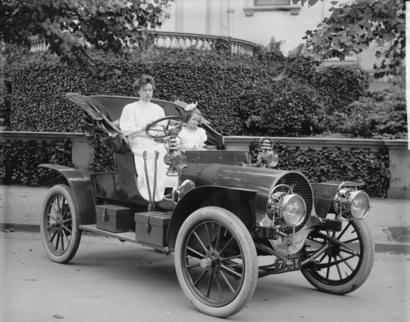
\includegraphics[width=\linewidth]{sample-franklin}
  \caption{1907 Franklin Model D roadster. Photograph by Harris \&
    Ewing, Inc. [Public domain], via Wikimedia
    Commons. (\url{https://goo.gl/VLCRBB}).}
\end{figure}

Your figures should contain a caption which describes the figure to
the reader. Figure captions go below the figure. Your figures should
also include a description suitable for screen readers, to
assist the visually-challenged to better understand your work.

Figure captions are placed below the figure.

\section{Citations and Bibliographies}

The use of Bib\TeX{} for the preparation and formatting of one's
references is strongly recommended. Authors' names should be complete
--- use full first names (``Donald E. Knuth'') not initials
(``D. E. Knuth'') --- and the salient identifying features of a
reference should be included: title, year, volume, number, pages,
article DOI, etc.

The bibliography is included in your source document with these two
commands, placed just before the \mintinline{latex}{\end{document}}
command:
\begin{minted}{latex}
\bibliography{bibfile}
\end{minted}
where ``\verb|bibfile|'' is the name, without the ``\verb|.bib|''
suffix, of the Bib\TeX{} file.


\subsection{Some examples}

A paginated journal article \cite{Abril07}, an enumerated journal
article \cite{Cohen07}, a reference to an entire issue
\cite{JCohen96}, a monograph (whole book) \cite{Kosiur01}, a
monograph/whole book in a series (see 2a in spec. document)
\cite{Harel79}, a divisible-book such as an anthology or compilation
\cite{Editor00} followed by the same example, however we only output
the series if the volume number is given \cite{Editor00a} (so series
should not be present since it has no vol. no.), a chapter in a
divisible book \cite{Spector90}, a chapter in a divisible book in a
series \cite{Douglass98}, a multi-volume work as book \cite{Knuth97},
an article in a proceedings (of a conference, symposium, workshop for
example) (paginated proceedings article) \cite{Andler79}, a
proceedings article with all possible elements \cite{Smith10}, an
example of an enumerated proceedings article \cite{VanGundy07}, an
informally published work \cite{Harel78}, a doctoral dissertation
\cite{Clarkson85}, a master's thesis: \cite{anisi03}, an online
document / world wide web resource \cite{Thornburg01, Ablamowicz07,
  Poker06}, a video game (Case 1) \cite{Obama08} and (Case 2)
\cite{Novak03} and \cite{Lee05} and (Case 3) a patent
\cite{JoeScientist001}, work accepted for publication \cite{rous08},
prolific author \cite{SaeediMEJ10} and \cite{SaeediJETC10}. Other
cites might contain `duplicate' DOI and URLs (some SIAM articles)
\cite{Kirschmer:2010:AEI:1958016.1958018}. Multi-volume works as books
\cite{MR781536} and \cite{MR781537}. A couple of citations with DOIs:
\cite{2004:ITE:1009386.1010128,Kirschmer:2010:AEI:1958016.1958018}. Online
citations: \cite{TUGInstmem, Thornburg01, R, UMassCitations}.

\section{Acknowledgments}

Identification of funding sources and other support, and thanks to
individuals and groups that assisted in the research and the
preparation of the work should be included in an acknowledgment
section, which is placed just before the reference section in your
document.

This section has a special environment:
\begin{minted}{latex}
\begin{acknowledgments}
  These are different acknowledgments.
\end{acknowledgments}
\end{minted}
so that the information contained therein can be more easily collected
during the article metadata extraction phase, and to ensure
consistency in the spelling of the section heading.

Authors should not prepare this section as a numbered or unnumbered
\mintinline{latex}{\section}; please use the ``\mintinline{latex}{acknowledgments}'' environment.

\section{Appendices}

If your work needs an appendix, add it before the
``\mintinline{latex}{\end{document}}'' command at the conclusion of your source
document.

Start the appendix with the ``\mintinline{latex}{\appendix}'' command:
\begin{minted}{latex}
\appendix
\end{minted}
and note that in the appendix, sections are lettered, not
numbered. 

%%
%% The acknowledgments section is defined using the "acknowledgments" environment
%% (and NOT an unnumbered section). This ensures the proper
%% identification of the section in the article metadata, and the
%% consistent spelling of the heading.
\begin{acknowledgments}
  Thanks to the developers of ACM consolidated LaTeX styles
  \url{https://github.com/borisveytsman/acmart} and to the developers
  of Elsevier updated \LaTeX{} templates
  \url{https://www.ctan.org/tex-archive/macros/latex/contrib/els-cas-templates}.  
\end{acknowledgments}

%%
%% Define the bibliography file to be used

%%
%% If your work has an appendix, this is the place to put it.

% \section{Online Resources}


% The sources for the ceur-art style are available via
% \begin{itemize}
% \item \href{https://github.com/yamadharma/ceurart}{GitHub},
% % \item \href{https://www.overleaf.com/project/5e76702c4acae70001d3bc87}{Overleaf},
% \item
%   \href{https://www.overleaf.com/latex/templates/template-for-submissions-to-ceur-workshop-proceedings-ceur-ws-dot-org/pkfscdkgkhcq}{Overleaf
%     template}.
% \end{itemize}


\bibliography{sample-ceur}
\end{document}

